\chapter{Background}
\lhead{\emph{Background}}

\section{Virtual Reality}

The term Virtual Reality (VR) refers to the generation of a 3D environment that can be interacted with by a user in a realistic fashion, with the aim of immersing the user in the environment as if it were the real world \cite{WhatVR}. While there are a large array of systems that can be considered VR, whenever the term is used in this report it is only referring to the head-mounted display (HMD) systems that have become popular in recent years with the release of the Oculus Rift \cite{Oculus} and the HTC Vive \cite{Vive} (Figure \ref{fig:Vive}). These are both consumer grade systems that are aimed at the immersive gaming market.

\begin{figure}[H]
    \begin{center}
    \begin{tabular}{ c c }
        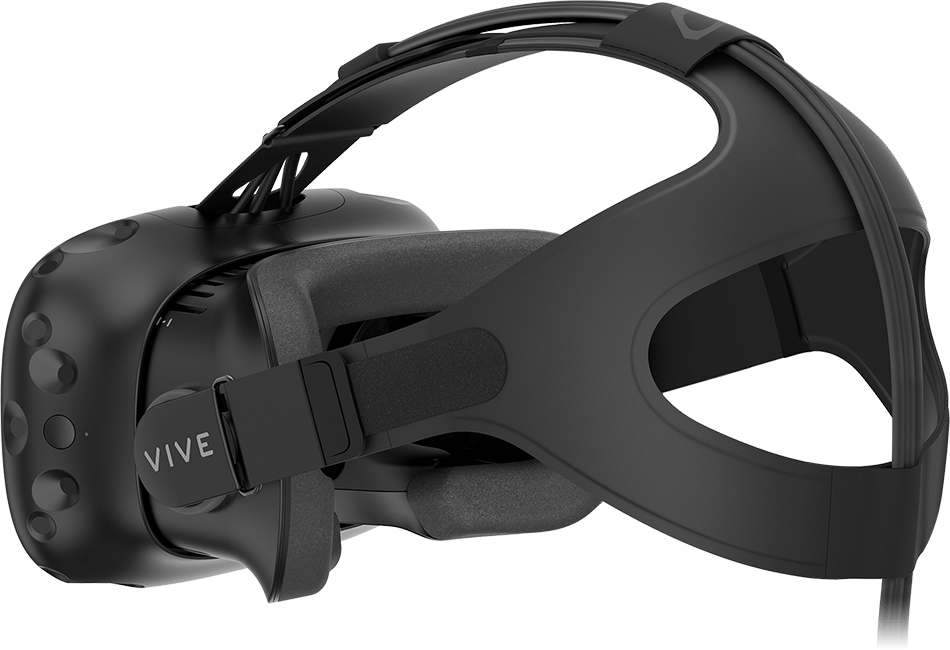
\includegraphics[width=0.4\textwidth]{Figures/vive.png} &
        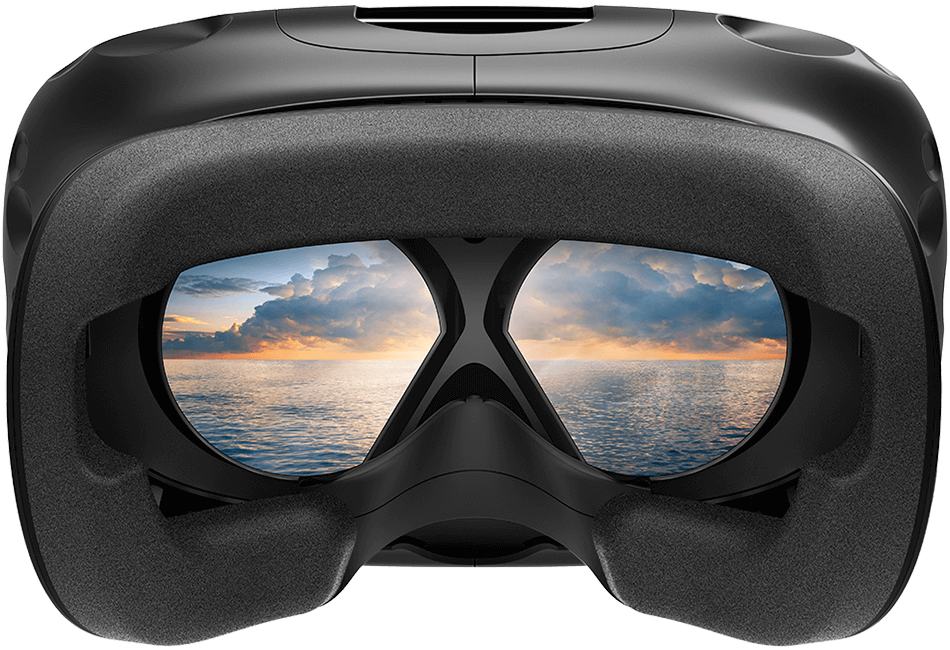
\includegraphics[width=0.4\textwidth]{Figures/vive2.png}
    \end{tabular}
    \caption[HTC Vive]{HTC Vive. Pictures of the Vive headset, reproduced from \cite{Vive}.}
    \label{fig:Vive}
    \end{center}
\end{figure}

HMD based systems display different images for each eye to provide the user with a sense of depth within the 3D environment, making the headset effectively operate like a pair of binoculars into the virtual world. The headset is also tracked in 3D space, and this movement translated into the 3D environment with very low latency. These features, among others, are all implemented with the aim of providing the user with presence within the virtual space that is comparable to observing the real world.

Due to its availability at the University of Southampton and in my own home, the HTC Vive was used as the VR device in the development and implementation of the teleoperations system discussed in this report. 

\section{Telerobotics}

A telerobot is a robot controlled from a distance by a human operator \cite{NAP4761}. Telerobots are typically developed to undertake activities within environments that are too dangerous or costly for humans to work in. Typical fields of telerobotics research include deep-space exploration \cite{fong2017interactive}, deep-sea exploration \cite{huvenne2018rovs}, and handling radioactive materials \cite{smith2017radiation}.

\subsection{VR in Telerobotics}
\label{subsection:VRTele}

The use of HMDs in teleoperations is not a new concept; NASA's Robonaut 2 was sent to the International Space Station in 2011 and can be controlled through a headset that displays the output of the robot's head cameras \cite{Robonaut}, and flying drones by First Person View (FPV), an analogue video feed transmitted over radio to a HMD, has become very popular in recent years \cite{FPV}. However, these systems are either incredibly expensive (Robonaut 2 is worth millions of dollars) or very limited (FPV systems are only capable of sending one low quality video stream over a short distance), and all suffer from the motion sickness issues discussed in Chapter \ref{chapter:intro}. While stereo camera FPV systems have been developed, so the user has depth perception and better presence in the drone's view, the motion sickness problem remains the major drawback of HMD based teleoperations systems \cite{2FPV}.

As previously established, motion sickness in VR is mitigated through high frame rates and low latency. However, typically VR based teleoperations systems are direct VR systems, so they display the video feeds provided by the telerobot's cameras directly in the headset. This entirely ties the frame rate and latency of the headset to the capabilities of the video transmission system, and only the most expensive and complicated systems will meet the strict requirements for comfortable VR and the spacial presence desired.

An alternate option to a direct system is an indirect system. This is one in which the video feed is abstracted from the headset in some way in the hope of providing improved comfort and awareness. Indirect systems can come in a variety of forms, such as placing the video feed on a virtual screen in the VR environment and controlling the robot using virtual controls laid out infront of the screen \cite{lipton2018baxter}, or a 3D map generated from a multi-line LiDAR and IMU \cite{wang2017novel} (Figure \ref{fig:VRTele}). These examples show the potential of indirect systems as a solution to VR based teleoperations, however neither of them provide true presence within their respective robots' environments. This project aims to contribute to this field of research by demonstrating an alternate approach to the problem that is capable of providing greater presence than these previous attempts.

\begin{figure}[H]
    \begin{center}
    \begin{tabular}{ c c }
        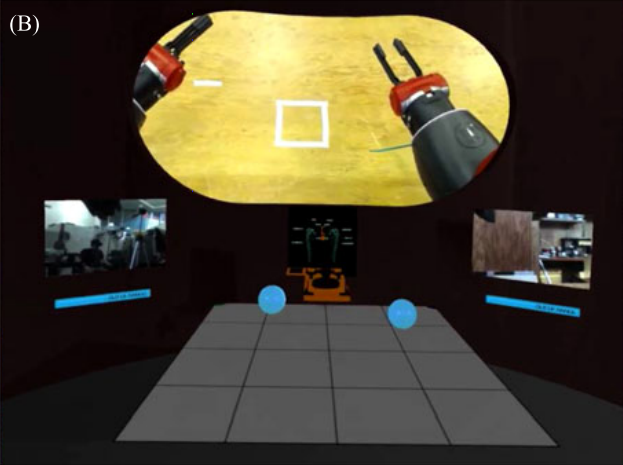
\includegraphics[width=0.45\textwidth]{Figures/homun.png} &
        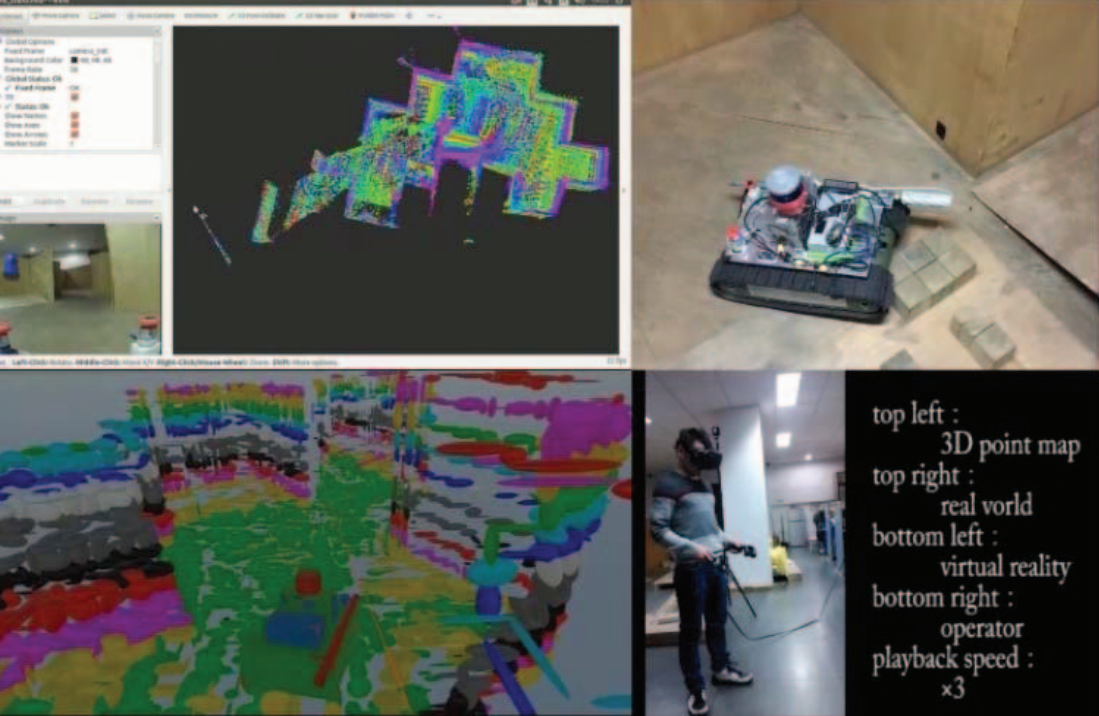
\includegraphics[width=0.5\textwidth]{Figures/lidar.png}
    \end{tabular}
    \caption[Indirect VR Teleoperations Examples]{Indirect VR Teleoperations Examples. A virtual control room based system (left) and a LiDAR 3D map based system (right), reproduced from \cite{lipton2018baxter} and \cite{wang2017novel}.}
    \label{fig:VRTele}
    \end{center}
\end{figure}

\section{Data Abstraction}
\label{Subsection:abstract}

\textit{Data abstraction} is the phrase that will be used in this report to describe the act of reducing an image down to only its most essential elements. It is similar in concept to an artist sketching a scene instead of attempting a full drawing. Comparing the concept to data compression is apt, as both aim to reduce the file size of the image, however data abstraction takes a very different approach to solving the problem than standard compression algorithms.

Data compression is the storing of information using a more space efficient encoding \cite{compression}. While some information is lost during lossy compression, the aim regardless of the algorithm used is to retain as much of the original information as possible. In contrast, the aim when utilising data abstraction is to discard all the information that is unnecessary to fulfilling the image's specific purpose. For example, if all that is required of an image is that basic shapes can be identified, then only the information on the boundaries of the shapes is necessary; the rest of the image can be discarded. An implementation of data abstraction can be seen in Figure \ref{fig:abstraction3rdyear}.

%\caption[My figure Title.]{My figure Title. Details how it was made. What is the point? Reproduced from}

\begin{figure}[H]
    \begin{center}
      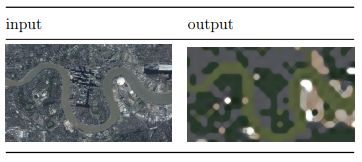
\includegraphics[width=0.6\textwidth]{Figures/abstraction3rdyear.png}
      \caption[Data Abstraction Example]{Data Abstraction Example. This is an abstraction of an aerial photograph of London, reproduced from \cite{abstraction3rdyear}.}
      \label{fig:abstraction3rdyear}
    \end{center}
\end{figure}

\section{Sobol Sequences}
\label{Subsection:sobol}

Sobol sequences are quasi-random sequences that were introduced to aid in approximating integrals. The aim is to form a sequence of points that are evenly spread across an S-dimensional unit cube \cite{joe2008constructing}, providing a much more even spread of points across the chosen space than can be produced from a pseudo-random number source (Figure \ref{fig:Sobol}). The code used in this project to produce these sequences was created by Leonhard Gr\"unschlo\ss\space \cite{CodeSource}.

\begin{figure}[H]
    \begin{center}
    \begin{tabular}{ c c }
        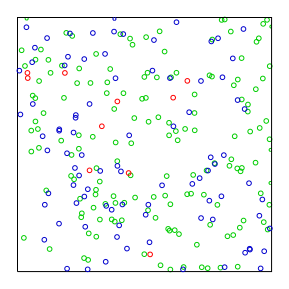
\includegraphics[width=0.33\textwidth]{Figures/Pseudorandom_sequence_2D.png} &
        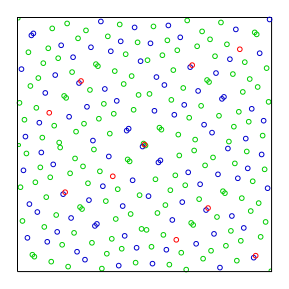
\includegraphics[width=0.33\textwidth]{Figures/Sobol_sequence_2D.png}
    \end{tabular}
    \caption[Comparison of Pseudo-Random and Quasi-Random Sequences]{Comparison of Pseudo-Random and Quasi-Random Sequences. 256 points from a pseudo-random generator (left) and 256 points from a Sobol sequence (right), reproduced from \cite{SobolWiki}.}
    \label{fig:Sobol}
    \end{center}
\end{figure}

\section{Computer Vision}

Computer vision is the automatic analysis of images and extraction of the useful information they contain \cite{CVDef}. A raw image is simply a large matrix of colour values, so for a computer to take action based on the contents of an image it must be able to recognise features using analysis of this data. Doing so involves many different techniques such as statistical pattern classification and geometric modelling \cite{ballard1982computer}. All computer vision methods in this project are implemented using the OpenCV libraries, and the example programs provided with them used as starting points for development \cite{OpenCV}.

\subsection{Edge Detection}
When attempting to recognise the features of an image, knowing the locations of the edges of objects within the scene is often very useful. An edge is defined as a significant local change in intensity, usually due to a discontinuity in either the intensity or its first derivative \cite{jain1995machine}. There are many algorithms available that will detect the edges of an image from the locations of these discontinuities. When the most popular algorithms (Laplacian of Gaussian, Robert, Prewitt, Sobel, and Canny) are compared \cite{maini2009study}, the most effective in almost all scenarios is Canny edge detection \cite{canny1986computational}, therefore this is the algorithm utilised in this project. Canny edge detection is demonstrated in Figure \ref{fig:canny1}.

\begin{figure}[H]
    \begin{center}
      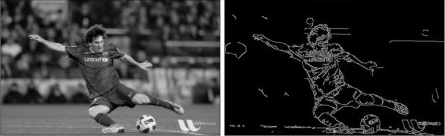
\includegraphics[width=0.9\textwidth]{Figures/canny2.png}
      \caption[Canny Edge Detection Example]{Canny Edge Detection Example. Simple edge detection program applied to a fairly detailed photo of Lionel Messi, to demonstrate its effectiveness with even complex images. Figure taken from an OpenCV Canny tutorial \cite{Canny1Source}.}
      \label{fig:canny1}
    \end{center}
\end{figure}

\subsection{Flood Filling}

Flood fill algorithms determine the area connected to a given cell (the seed point) in a multi-dimensional array that have similar intensity values for the purpose of filling them with a chosen colour \cite{FloodFill}. This is a technique that is not only useful in image processing, but also for many other fields such as in passive acoustic monitoring, where finding the area connected to a given node can be useful as part of tracking in 4D space (x,y,z,time) \cite{nosal2008flood}. A demonstration of flood fill has been presented in Figure \ref{fig:EgFloodFill}.

\begin{figure}[H]
    \begin{center}
    \begin{tabular}{ c c }
        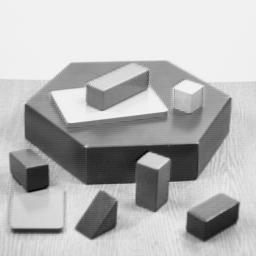
\includegraphics[width=0.35\textwidth]{Figures/blox.jpg} &
        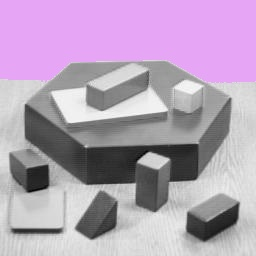
\includegraphics[width=0.35\textwidth]{Figures/bloxFilled.jpg}
    \end{tabular}
    \caption[Flood Filling Example]{Flood Filling Example. The original image (left) was provided by OpenCV \cite{OpenCV}. The right image is the result of flood filling from the top left corner.}
    \label{fig:EgFloodFill}
    \end{center}
\end{figure}

\subsection{Depth Mapping}
\label{subsection:depth}

The main component in the human brain's perception of 3D is the identification of disparity between the locations of objects in the 2D images being produced by our eyes \cite{qian1997binocular}. The greater the difference in the horizontal placement of an object between the images, the closer the object to the observer. This technique can be used in computer vision to produce depth/disparity maps. Depth maps display differences in depth as a gradient from white to black (Figure \ref{fig:depthmap}), and can be produced using a variety of different algorithms. The most common are block matching algorithms, which use simple geometry and the matching of blocks of pixels horizontally in the 2 images to calculate depth \cite{linda2001stockman}. For these algorithms to locate the same object in different places in the 2 images, the cameras taking them must be calibrated to rectify any distortion due to the lenses \cite{distort} or discrepancies in the mounting that would cause them to be out of line \cite{stereocal}. Without this image rectification, the similar blocks the algorithm is attempting to locate will not be on the same horizontal row or will be distorted, so the algorithm will produce a mostly black image.

\begin{figure}[H]
    \begin{center}
      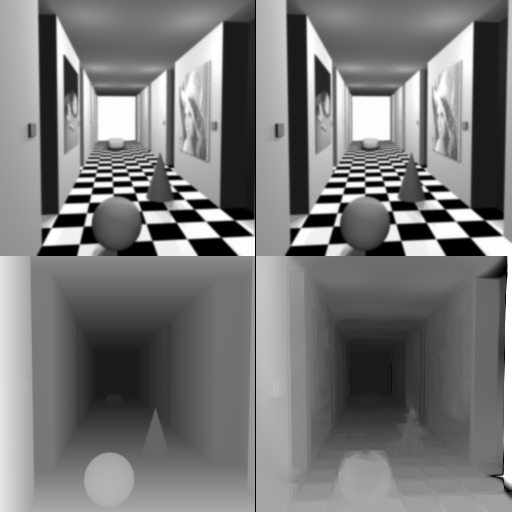
\includegraphics[width=0.8\textwidth]{Figures/depthmap.png}
      \caption[Depth Mapping Example]{Depth Mapping Example. A stereo pair of images, with their exact disparity map bottom left and a disparity map produced by a dense disparity estimation algorithm bottom right- reproduced from \cite{deptheg}.}
      \label{fig:depthmap}
    \end{center}
\end{figure}

\section{Wireless Communication}

The different methods of wireless communication available for a telerobotics system have varying requirements and benefits. For instance, the analogue video transmission found in FPV drone flying (as mentioned in Section \ref{subsection:VRTele}) is low latency at the expensive of video quality, range, and communication outside of line of sight. This is acceptable for flying a drone in an open field, but would not be adequate for controlling a telerobot from a VR headset in a completely different room as is the aim of this project. A better choice of communication method would be over Wi-Fi, as it allows for communication across significantly longer distances and outside of line of sight. The trade off is an acceptable increase in latency.

The two most common Wi-Fi communication protocols are TCP (Transmission Control Protocol) and UDP (User Datagram Protocol). TCP is a connection-oriented protocol, so uses handshaking to guarantee reliable and ordered transfer of data \cite{fall2011tcp}. The trade off to this is that the handshaking slows down the process of communication. UDP does not include this handshaking, so there is no guarantee that the packets will arrive, however they are sent with minimal overheads \cite{postel1980user}. UDP is therefore the optimal choice for a system where throughput is of higher priority then packet reliability and ordering, such as the system presented by this report- images not arriving in the correct order and the ocassional loss of packets would not have a significant effect on the functionality of the system in comparison to the usability improvement a reduction in latency provides.